\documentclass{article}

\usepackage[utf8]{inputenc}
\usepackage[margin=1in]{geometry}
\usepackage{amsmath, amssymb, amsthm}
% enumitem not available in this TeX installation
\usepackage{hyperref}
\usepackage{booktabs}
\usepackage{tikz}
\usetikzlibrary{arrows.meta, positioning, calc}

% --- Theorem environments ---
\newtheorem{theorem}{Theorem}[section]
\newtheorem{lemma}[theorem]{Lemma}
\newtheorem{corollary}[theorem]{Corollary}
\newtheorem{definition}[theorem]{Definition}
\newtheorem{example}{Example}[section]

\theoremstyle{remark}
\newtheorem*{remark}{Remark}

% --- Indent subsection headings and content ---
\newlength{\subsecindent}
\setlength{\subsecindent}{2em}

\makeatletter
\renewcommand\subsection{\@startsection{subsection}{2}{\subsecindent}%
  {-3.25ex\@plus -1ex \@minus -.2ex}%
  {1.5ex \@plus .2ex}%
  {\normalfont\large\bfseries}}
\makeatother

\newenvironment{sub}{%
  \begin{list}{}{%
    \setlength{\leftmargin}{4em}%
    \setlength{\rightmargin}{0pt}%
    \setlength{\topsep}{0pt}%
    \setlength{\partopsep}{0pt}%
    \setlength{\parsep}{\parskip}%
    \setlength{\itemsep}{\parskip}%
  }\item\relax
}{\end{list}}

\newenvironment{secbody}{%
  \begin{list}{}{%
    \setlength{\leftmargin}{\subsecindent}%
    \setlength{\rightmargin}{0pt}%
    \setlength{\topsep}{0pt}%
    \setlength{\partopsep}{0pt}%
    \setlength{\parsep}{\parskip}%
    \setlength{\itemsep}{\parskip}%
  }\item\relax
}{\end{list}}

% --- Custom commands ---
\newcommand{\Prob}{\mathbb{P}}
\newcommand{\given}{\mid}

\title{Floating-point}
\author{Reo Tajiri}
\date{\today}

\begin{document}
\maketitle
\tableofcontents
\newpage

%=============================================================================
% SECTION 1: Introduction
%=============================================================================
\section{Introduction}

\begin{secbody}
Computers must represent real numbers, not just integers.
Many applications---physics simulations, graphics, scientific computing,
financial modeling---require fractional values and very large or very small
magnitudes.

\textbf{Fixed-point} representations allocate a fixed number of bits for the
integer and fractional parts.  This limits both range and precision
simultaneously: you cannot represent both $0.00001$ and $1{,}000{,}000$ without
wasting bits.

\textbf{Floating-point} solves this by adopting the idea of scientific
notation:
\[
  (-1)^{s} \times M \times 2^{E}
\]
where $s$ is the sign, $M$ is the significand (mantissa), and $E$ is the
exponent.  This trades a \emph{fixed} number of significant digits for an
enormous dynamic range.
\end{secbody}

%=============================================================================
% SECTION 2: Number Representation Review
%=============================================================================
\section{Number Representation Review}

\subsection{Binary Fractions}
\begin{sub}
Just as decimal fractions use negative powers of 10, binary fractions use
negative powers of 2:
\[
  (0.b_1 b_2 b_3 \ldots)_2
  = b_1 \times 2^{-1} + b_2 \times 2^{-2} + b_3 \times 2^{-3} + \cdots
\]

\begin{example}
$0.101_2 = 1\times2^{-1} + 0\times2^{-2} + 1\times2^{-3}
          = 0.5 + 0 + 0.125 = 0.625_{10}$.
\end{example}

\begin{example}
$5.75_{10}$: The integer part is $101_2$. For the fractional part $0.75$:
$0.75\times2=1.5$ (take 1), $0.5\times2=1.0$ (take 1).  So $5.75_{10} =
101.11_2$.
\end{example}
\end{sub}

\subsection{Scientific Notation Analogy}
\begin{sub}
In decimal scientific notation:
\[
  6.022 \times 10^{23}
\]
The \emph{significand} is $6.022$ and the \emph{exponent} is $23$.  IEEE~754
floating-point works identically but in base~2:
\[
  1.0110\ldots \times 2^{n}
\]
The leading $1$ is implicit (for normalized numbers), saving one bit of
storage.
\end{sub}

%=============================================================================
% SECTION 3: IEEE 754 Standard
%=============================================================================
\section{IEEE 754 Standard}

\begin{secbody}
The IEEE~754 standard (1985, revised 2008/2019) defines formats, rounding
rules, and special values for floating-point arithmetic.  The two most common
formats are \textbf{single precision} (32-bit) and \textbf{double precision}
(64-bit).
\end{secbody}

\subsection{Single Precision (32-bit)}
\begin{sub}
\begin{center}
\begin{tabular}{lccc}
\toprule
Field & Sign & Exponent & Fraction \\
\midrule
Bits  & 1    & 8        & 23       \\
Bit positions & [31] & [30:23] & [22:0] \\
\bottomrule
\end{tabular}
\end{center}

\begin{center}
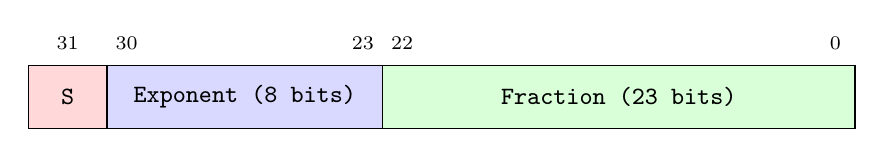
\begin{tikzpicture}[
  box/.style={draw, minimum height=0.8cm, font=\ttfamily\small},
]
\node[box, minimum width=1cm,   fill=red!15]   (S) at (0,0)    {S};
\node[box, minimum width=3.5cm, fill=blue!15]  (E) at (2.25,0) {Exponent (8 bits)};
\node[box, minimum width=6cm,   fill=green!15] (F) at (7,0)    {Fraction (23 bits)};

\node[font=\scriptsize, above=2pt] at (S.north) {31};
\node[font=\scriptsize, above=2pt] at ([xshift=-1.5cm]E.north) {30};
\node[font=\scriptsize, above=2pt] at ([xshift=1.5cm]E.north) {23};
\node[font=\scriptsize, above=2pt] at ([xshift=-2.75cm]F.north) {22};
\node[font=\scriptsize, above=2pt] at ([xshift=2.75cm]F.north) {0};
\end{tikzpicture}
\end{center}

\textbf{Value} (normalized): $(-1)^{s}\times 1.\text{fraction}\times 2^{(\text{exponent} - 127)}$

Exponent range: $1$ to $254$ (0 and 255 are reserved for special values).
\end{sub}

\subsection{Double Precision (64-bit)}
\begin{sub}
\begin{center}
\begin{tabular}{lccc}
\toprule
Field & Sign & Exponent & Fraction \\
\midrule
Bits  & 1    & 11       & 52       \\
Bit positions & [63] & [62:52] & [51:0] \\
\bottomrule
\end{tabular}
\end{center}

\begin{center}
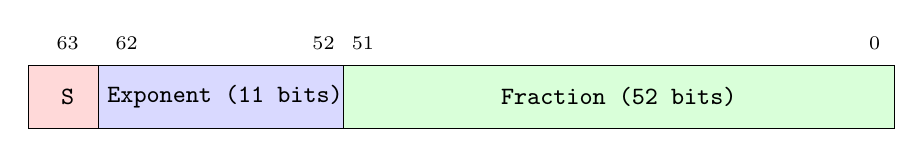
\begin{tikzpicture}[
  box/.style={draw, minimum height=0.8cm, font=\ttfamily\small},
]
\node[box, minimum width=1cm,   fill=red!15]   (S) at (0,0)    {S};
\node[box, minimum width=3cm,   fill=blue!15]  (E) at (2,0)    {Exponent (11 bits)};
\node[box, minimum width=7cm,   fill=green!15] (F) at (7,0)    {Fraction (52 bits)};

\node[font=\scriptsize, above=2pt] at (S.north) {63};
\node[font=\scriptsize, above=2pt] at ([xshift=-1.25cm]E.north) {62};
\node[font=\scriptsize, above=2pt] at ([xshift=1.25cm]E.north) {52};
\node[font=\scriptsize, above=2pt] at ([xshift=-3.25cm]F.north) {51};
\node[font=\scriptsize, above=2pt] at ([xshift=3.25cm]F.north) {0};
\end{tikzpicture}
\end{center}

\textbf{Value} (normalized): $(-1)^{s}\times 1.\text{fraction}\times 2^{(\text{exponent} - 1023)}$

Exponent range: $1$ to $2046$ (0 and 2047 are reserved for special values).
\end{sub}

%=============================================================================
% SECTION 4: Components Explained
%=============================================================================
\section{Components Explained}

\subsection{Sign Bit}
\begin{sub}
\begin{center}
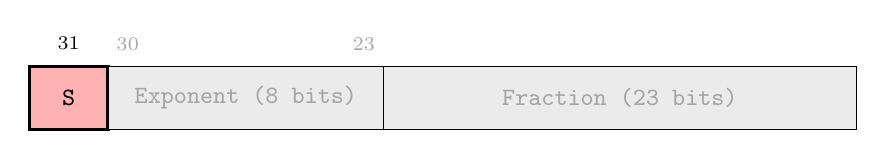
\begin{tikzpicture}[
  box/.style={draw, minimum height=0.8cm, font=\ttfamily\small},
]
\node[box, minimum width=1cm,   fill=red!30, line width=1.2pt] (S) at (0,0) {S};
\node[box, minimum width=3.5cm, fill=black!8, text=black!35]  (E) at (2.25,0) {Exponent (8 bits)};
\node[box, minimum width=6cm,   fill=black!8, text=black!35]  (F) at (7,0)    {Fraction (23 bits)};

\node[font=\scriptsize, above=2pt] at (S.north) {31};
\node[font=\scriptsize, color=black!35, above=2pt] at ([xshift=-1.5cm]E.north) {30};
\node[font=\scriptsize, color=black!35, above=2pt] at ([xshift=1.5cm]E.north) {23};

\end{tikzpicture}
\end{center}

\begin{itemize}
  \item $s = 0$: positive number
  \item $s = 1$: negative number
\end{itemize}
This applies to all values, including zero (IEEE~754 has both $+0$ and $-0$).
\end{sub}

\subsection{Biased Exponent}
\begin{sub}
\begin{center}
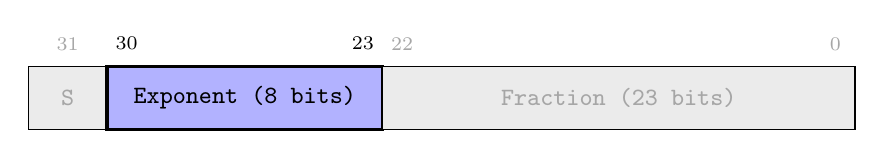
\begin{tikzpicture}[
  box/.style={draw, minimum height=0.8cm, font=\ttfamily\small},
]
\node[box, minimum width=1cm,   fill=black!8, text=black!35]   (S) at (0,0)    {S};
\node[box, minimum width=3.5cm, fill=blue!30, line width=1.2pt] (E) at (2.25,0) {Exponent (8 bits)};
\node[box, minimum width=6cm,   fill=black!8, text=black!35]   (F) at (7,0)    {Fraction (23 bits)};

\node[font=\scriptsize, color=black!35, above=2pt] at (S.north) {31};
\node[font=\scriptsize, above=2pt] at ([xshift=-1.5cm]E.north) {30};
\node[font=\scriptsize, above=2pt] at ([xshift=1.5cm]E.north) {23};
\node[font=\scriptsize, color=black!35, above=2pt] at ([xshift=-2.75cm]F.north) {22};
\node[font=\scriptsize, color=black!35, above=2pt] at ([xshift=2.75cm]F.north) {0};
\end{tikzpicture}
\end{center}

The exponent field stores $E + \text{bias}$, not the true exponent $E$ itself.
Using a bias (instead of two's complement) simplifies hardware comparisons,
because the stored exponent can be compared as an unsigned integer.

\begin{center}
\begin{tabular}{lcc}
\toprule
Format & Bias & True exponent range \\
\midrule
Single (8-bit exp) & 127 & $-126$ to $+127$ \\
Double (11-bit exp) & 1023 & $-1022$ to $+1023$ \\
\bottomrule
\end{tabular}
\end{center}

To compute the true exponent, add $-127$ (in two's complement) to the stored
exponent:
\begin{align*}
  127_{10}  &= 0\;1111111_2 \\
  -127_{10} &= 1\;0000001_2 \quad \text{(8-bit two's complement)}
\end{align*}

\begin{example}
If the stored exponent byte is $1000\;0100_2$, the true exponent is
obtained by adding $-127$ ($1000\;0001_2$) directly in binary:
\[
  \begin{array}{r}
       1000\;0100 \\
    +  1000\;0001 \\
    \hline
    \tikz[baseline=(X.base)]{\node[inner sep=1pt](X){$1$};\draw[red, thick](X.south west)--(X.north east);}\;0000\;0101
  \end{array}
\]
The leading $1$ is the 9th bit (overflow carry) and is discarded, leaving
the 8-bit result $0000\;0101_2 = 5$.
\end{example}
\end{sub}

\subsection{Implicit Leading 1 and Significand}
\begin{sub}
\begin{center}
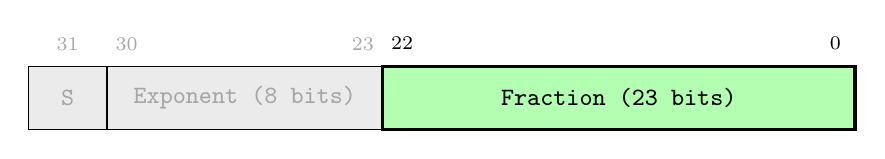
\begin{tikzpicture}[
  box/.style={draw, minimum height=0.8cm, font=\ttfamily\small},
]
\node[box, minimum width=1cm,   fill=black!8, text=black!35]   (S) at (0,0)    {S};
\node[box, minimum width=3.5cm, fill=black!8, text=black!35]   (E) at (2.25,0) {Exponent (8 bits)};
\node[box, minimum width=6cm,   fill=green!30, line width=1.2pt] (F) at (7,0)  {Fraction (23 bits)};

\node[font=\scriptsize, color=black!35, above=2pt] at (S.north) {31};
\node[font=\scriptsize, color=black!35, above=2pt] at ([xshift=-1.5cm]E.north) {30};
\node[font=\scriptsize, color=black!35, above=2pt] at ([xshift=1.5cm]E.north) {23};
\node[font=\scriptsize, above=2pt] at ([xshift=-2.75cm]F.north) {22};
\node[font=\scriptsize, above=2pt] at ([xshift=2.75cm]F.north) {0};
\end{tikzpicture}
\end{center}

For normalized numbers, the significand is $1.\text{fraction}$.  The leading
$1$ is \emph{not stored}---it is implicit.  This gives one extra bit of
precision for free.

\begin{example}
If the fraction field stores $1010\;0000\;0000\;0000\;0000\;000$, the
implicit leading 1 is prepended:
\[
  \underbrace{1}_{\text{implicit}}.\underbrace{1010\;0000\;0000\;0000\;0000\;000}_{\text{stored fraction (23 bits)}}
\]
The full significand is:
\[
  1.101_2 = 1 + \frac{1}{2} + \frac{0}{4} + \frac{1}{8}
           = 1 + 0.5 + 0 + 0.125 = 1.625_{10}
\]
\end{example}

\begin{definition}[Significand vs.\ Mantissa]
Strictly, IEEE~754 uses the term \textbf{significand} (the full value
$1.\text{fraction}$).  The stored bits are the \textbf{fraction} (or
\textbf{trailing significand}).  The older term ``mantissa'' is sometimes used
informally but technically refers to the fractional part of a logarithm.
\end{definition}
\end{sub}

%=============================================================================
% SECTION 5: Conversion Procedures
%=============================================================================
\section{Conversion Procedures}

\subsection{Decimal to IEEE 754 (Single Precision)}
\begin{sub}
\textbf{Algorithm:}
\begin{enumerate}
  \item Determine the \textbf{sign bit}: $s=0$ if positive, $s=1$ if negative.
        Work with the absolute value from here.
  \item Convert the \textbf{integer part} to binary (repeated division by 2).
  \item Convert the \textbf{fractional part} to binary (repeated multiplication
        by 2).
  \item Combine and write in normalized form $1.xxxxx \times 2^{E}$.
  \item Compute the \textbf{biased exponent}: stored exponent $= E + 127$.
        Convert to 8-bit binary.
  \item The bits after the binary point are the \textbf{fraction field} (pad or
        truncate to 23 bits).
\end{enumerate}

\begin{example}[Convert $-6.625_{10}$ to IEEE 754 single precision]
\leavevmode
\begin{enumerate}
  \item Sign: negative $\Rightarrow s = 1$.
  \item Integer part $6 = 110_2$.
  \item Fractional part $0.625$:
        $0.625\times2=1.25$ (1),
        $0.25\times2=0.5$ (0),
        $0.5\times2=1.0$ (1).
        So $0.625_{10} = 0.101_2$.
  \item Combined: $110.101_2 = 1.10101 \times 2^{2}$.
  \item Biased exponent: $2 + 127 = 129 = 10000001_2$.
  \item Fraction: $10101\underbrace{000\ldots0}_{18\text{ zeros}}$.
\end{enumerate}

Final 32-bit representation:
\[
  \underbrace{1}_{\text{sign}}\;\;
  \underbrace{10000001}_{\text{exponent}}\;\;
  \underbrace{10101000000000000000000}_{\text{fraction}}
\]
In hexadecimal: \texttt{0xC0D40000}.
\end{example}
\end{sub}

\subsection{IEEE 754 to Decimal}
\begin{sub}
\textbf{Algorithm:}
\begin{enumerate}
  \item Extract the sign bit $s$, exponent field $E_{\text{stored}}$, and
        fraction bits.
  \item Compute the true exponent: $E = E_{\text{stored}} - \text{bias}$.
  \item Reconstruct the significand: $M = 1.\text{fraction}_2$.
  \item Compute the value: $(-1)^s \times M \times 2^E$.
\end{enumerate}

\begin{example}[Convert \texttt{0x41C80000} to decimal]
Binary: \texttt{0100\,0001\,1100\,1000\,0000\,0000\,0000\,0000}.
\begin{enumerate}
  \item Sign bit: $s = 0$ (positive).
  \item Exponent: $10000011_2 = 131$. True exponent: $131 - 127 = 4$.
  \item Fraction bits: $10010000\ldots0$.
        Significand: $M = 1.10010_2$.
  \item Value: $+1.10010_2 \times 2^{4} = 11001.0_2 = 25.0_{10}$.
\end{enumerate}
\end{example}
\end{sub}

%=============================================================================
% SECTION 6: Special Values
%=============================================================================
\section{Special Values}

\begin{secbody}
IEEE~754 reserves certain exponent values to encode special numbers.
\end{secbody}

\subsection{Zero}
\begin{sub}
\begin{itemize}
  \item Exponent $= 0$, Fraction $= 0$.
  \item Both $+0$ (sign $=0$) and $-0$ (sign $=1$) exist.
  \item By definition, $+0 = -0$ in comparisons.
\end{itemize}
\end{sub}

\subsection{Infinity}
\begin{sub}
\begin{itemize}
  \item Exponent $=$ all 1s (255 for single, 2047 for double), Fraction $= 0$.
  \item $+\infty$: sign $= 0$; \quad $-\infty$: sign $= 1$.
  \item Results from overflow or division by zero (e.g., $1.0 / 0.0 = +\infty$).
\end{itemize}
\end{sub}

\subsection{NaN (Not a Number)}
\begin{sub}
\begin{itemize}
  \item Exponent $=$ all 1s, Fraction $\neq 0$.
  \item Results from invalid operations: $0/0$, $\sqrt{-1}$, $\infty - \infty$.
  \item \textbf{Quiet NaN (qNaN)}: propagates through computations silently.
        Fraction's most significant bit is 1.
  \item \textbf{Signaling NaN (sNaN)}: raises an exception when used.
        Fraction's most significant bit is 0 (with at least one other fraction
        bit set).
  \item Any comparison involving NaN returns false
        (including $\text{NaN} = \text{NaN}$).
\end{itemize}
\end{sub}

\subsection{Denormalized (Subnormal) Numbers}
\begin{sub}
\begin{itemize}
  \item Exponent $= 0$, Fraction $\neq 0$.
  \item No implicit leading 1; the significand is $0.\text{fraction}$.
  \item True exponent is fixed at $-126$ (single) or $-1022$ (double).
  \item Fills the gap between zero and the smallest normalized number,
        providing \textbf{gradual underflow}.
\end{itemize}

Value: $(-1)^s \times 0.\text{fraction} \times 2^{-126}$ \quad (single precision).
\end{sub}

\subsection{Summary Table (Single Precision)}
\begin{sub}
\begin{center}
\begin{tabular}{llll}
\toprule
\textbf{Exponent} & \textbf{Fraction} & \textbf{Value} & \textbf{Category} \\
\midrule
0        & 0        & $\pm 0$                                                & Zero \\
0        & $\neq 0$ & $(-1)^s\times 0.\text{frac}\times 2^{-126}$           & Denormalized \\
1--254   & anything & $(-1)^s\times 1.\text{frac}\times 2^{E-127}$          & Normalized \\
255      & 0        & $\pm\infty$                                            & Infinity \\
255      & $\neq 0$ & NaN                                                    & Not a Number \\
\bottomrule
\end{tabular}
\end{center}
\end{sub}

%=============================================================================
% SECTION 7: Floating-Point Arithmetic
%=============================================================================
\section{Floating-Point Arithmetic}

\subsection{Addition and Subtraction}
\begin{sub}
\textbf{Algorithm:}
\begin{enumerate}
  \item \textbf{Align exponents}: shift the significand of the smaller number
        right until both exponents match.
  \item \textbf{Add/subtract significands}: operate on the aligned significands
        according to the signs.
  \item \textbf{Normalize}: shift the result so it is in the form
        $1.xxx \times 2^E$.  Adjust the exponent accordingly.
  \item \textbf{Round}: apply the rounding rule (typically round to nearest,
        ties to even).
  \item \textbf{Check} for overflow/underflow.
\end{enumerate}

\begin{example}[Compute $1.5 + 3.25$ in floating-point]
\leavevmode
\begin{enumerate}
  \item $1.5 = 1.1_2 \times 2^{0}$, \quad $3.25 = 1.101_2 \times 2^{1}$.
  \item Align: shift $1.1_2$ right by 1 $\Rightarrow 0.11_2 \times 2^{1}$.
  \item Add significands: $0.110_2 + 1.101_2 = 10.011_2$.
  \item Normalize: $10.011_2 \times 2^{1} = 1.0011_2 \times 2^{2}$.
  \item Result: $1.0011_2 \times 2^{2} = 100.11_2 = 4.75_{10}$. \checkmark
\end{enumerate}
\end{example}
\end{sub}

\subsection{Multiplication}
\begin{sub}
\textbf{Algorithm:}
\begin{enumerate}
  \item \textbf{Sign}: $s_{\text{result}} = s_1 \oplus s_2$ (XOR of sign bits).
  \item \textbf{Exponent}: $E_{\text{result}} = E_1 + E_2$.
        (When using biased exponents: add biased values and subtract the bias
        once.)
  \item \textbf{Significands}: multiply $M_1 \times M_2$.  The product of two
        values in $[1,2)$ lies in $[1,4)$.
  \item \textbf{Normalize}: if the product $\geq 2.0$, shift right by 1 and
        increment the exponent.
  \item \textbf{Round} and check for overflow/underflow.
\end{enumerate}

\begin{example}[Compute $-1.5 \times 2.5$]
\leavevmode
\begin{enumerate}
  \item $-1.5 = -1.1_2\times 2^0$, \quad $2.5 = 1.01_2\times 2^1$.
  \item Sign: $1 \oplus 0 = 1$ (negative).
  \item Exponent: $0 + 1 = 1$.
  \item Significands: $1.1_2 \times 1.01_2 = 1.111_2$.
  \item $1.111_2 < 2$, already normalized.
  \item Result: $-1.111_2 \times 2^{1} = -11.11_2 = -3.75_{10}$. \checkmark
\end{enumerate}
\end{example}
\end{sub}

%=============================================================================
% SECTION 8: Rounding
%=============================================================================
\section{Rounding}

\subsection{Round to Nearest, Ties to Even (Default)}
\begin{sub}
IEEE~754's default rounding mode:
\begin{itemize}
  \item Round to the nearest representable value.
  \item If the value is exactly halfway between two representable numbers,
        round to the one whose least significant bit is \textbf{0} (i.e.,
        the even one).
\end{itemize}

This avoids systematic upward or downward bias that would accumulate over many
operations.

\begin{example}
If the representable values are $1.00_2$ and $1.01_2$, and the exact result
is $1.001_2$ (exactly halfway), we round to $1.00_2$ (even) rather than
$1.01_2$ (odd).
\end{example}
\end{sub}

\subsection{Other Rounding Modes}
\begin{sub}
IEEE~754 defines three additional rounding modes:
\begin{center}
\begin{tabular}{ll}
\toprule
\textbf{Mode} & \textbf{Description} \\
\midrule
Round toward $+\infty$ & Always round up (ceiling) \\
Round toward $-\infty$ & Always round down (floor) \\
Round toward zero      & Truncate (chop toward zero) \\
\bottomrule
\end{tabular}
\end{center}
These are used in interval arithmetic and for specific numerical algorithms.
\end{sub}

\subsection{Precision Loss and Guard/Round/Sticky Bits}
\begin{sub}
During arithmetic, extra bits are maintained beyond the stored precision to
improve rounding accuracy:
\begin{itemize}
  \item \textbf{Guard bit}: first extra bit beyond the stored fraction.
  \item \textbf{Round bit}: second extra bit.
  \item \textbf{Sticky bit}: OR of all remaining bits beyond the round bit.
        Once set to 1, it stays 1.
\end{itemize}

These three bits together let the hardware determine the correct rounding
direction without storing the full intermediate result.
\end{sub}

%=============================================================================
% SECTION 9: Floating-Point in MIPS
%=============================================================================
\section{Floating-Point in MIPS}

\subsection{Coprocessor 1 and FP Registers}
\begin{sub}
MIPS handles floating-point via \textbf{Coprocessor 1 (CP1)}, which has its
own register file:
\begin{itemize}
  \item 32 FP registers: \texttt{\$f0}--\texttt{\$f31} (each 32 bits wide).
  \item \textbf{Single precision}: each \texttt{\$f}$n$ holds one 32-bit float.
  \item \textbf{Double precision}: an even-odd pair \texttt{\$f}$n$/\texttt{\$f}$(n{+}1)$
        holds one 64-bit double.  By convention, reference the even register
        (e.g., \texttt{\$f0} means the pair \texttt{\$f0}/\texttt{\$f1}).
\end{itemize}
\end{sub}

\subsection{Key MIPS FP Instructions}
\begin{sub}
\begin{center}
\begin{tabular}{lll}
\toprule
\textbf{Instruction} & \textbf{Meaning} & \textbf{Example} \\
\midrule
\texttt{add.s fd, fs, ft} & $\texttt{fd} = \texttt{fs} + \texttt{ft}$ (single) & \texttt{add.s \$f2, \$f4, \$f6} \\
\texttt{sub.s fd, fs, ft} & $\texttt{fd} = \texttt{fs} - \texttt{ft}$ (single) & \texttt{sub.s \$f2, \$f4, \$f6} \\
\texttt{mul.s fd, fs, ft} & $\texttt{fd} = \texttt{fs} \times \texttt{ft}$ (single) & \texttt{mul.s \$f2, \$f4, \$f6} \\
\texttt{div.s fd, fs, ft} & $\texttt{fd} = \texttt{fs} / \texttt{ft}$ (single) & \texttt{div.s \$f2, \$f4, \$f6} \\
\midrule
\texttt{add.d fd, fs, ft} & double-precision add & \texttt{add.d \$f0, \$f2, \$f4} \\
\texttt{sub.d fd, fs, ft} & double-precision subtract & \texttt{sub.d \$f0, \$f2, \$f4} \\
\texttt{mul.d fd, fs, ft} & double-precision multiply & \texttt{mul.d \$f0, \$f2, \$f4} \\
\texttt{div.d fd, fs, ft} & double-precision divide & \texttt{div.d \$f0, \$f2, \$f4} \\
\midrule
\texttt{lwc1 ft, offset(rs)} & load word to FP register & \texttt{lwc1 \$f0, 0(\$t0)} \\
\texttt{swc1 ft, offset(rs)} & store word from FP register & \texttt{swc1 \$f0, 0(\$t0)} \\
\texttt{ldc1 ft, offset(rs)} & load double to FP pair & \texttt{ldc1 \$f0, 0(\$t0)} \\
\texttt{sdc1 ft, offset(rs)} & store double from FP pair & \texttt{sdc1 \$f0, 0(\$t0)} \\
\midrule
\texttt{mtc1 rt, fs} & move from GPR to FP register & \texttt{mtc1 \$t0, \$f0} \\
\texttt{mfc1 rt, fs} & move from FP register to GPR & \texttt{mfc1 \$t0, \$f0} \\
\texttt{cvt.s.w fd, fs} & convert int to single & \texttt{cvt.s.w \$f0, \$f1} \\
\texttt{cvt.d.s fd, fs} & convert single to double & \texttt{cvt.d.s \$f0, \$f2} \\
\bottomrule
\end{tabular}
\end{center}
\end{sub}

\subsection{FP Comparison and Branching}
\begin{sub}
MIPS FP comparisons set a \textbf{condition flag} in CP1 (not a GPR).
Branch instructions then test this flag.

\begin{center}
\begin{tabular}{ll}
\toprule
\textbf{Instruction} & \textbf{Meaning} \\
\midrule
\texttt{c.eq.s fs, ft} & set flag if $\texttt{fs} = \texttt{ft}$ (single) \\
\texttt{c.lt.s fs, ft} & set flag if $\texttt{fs} < \texttt{ft}$ (single) \\
\texttt{c.le.s fs, ft} & set flag if $\texttt{fs} \leq \texttt{ft}$ (single) \\
\texttt{c.eq.d fs, ft} & set flag if $\texttt{fs} = \texttt{ft}$ (double) \\
\texttt{c.lt.d fs, ft} & set flag if $\texttt{fs} < \texttt{ft}$ (double) \\
\texttt{c.le.d fs, ft} & set flag if $\texttt{fs} \leq \texttt{ft}$ (double) \\
\midrule
\texttt{bc1t label} & branch if FP condition flag is \textbf{true} \\
\texttt{bc1f label} & branch if FP condition flag is \textbf{false} \\
\bottomrule
\end{tabular}
\end{center}

\begin{example}[Branch if \texttt{\$f0} $<$ \texttt{\$f2} (single)]
\begin{verbatim}
      c.lt.s  $f0, $f2    # set flag if $f0 < $f2
      bc1t    less_than    # branch if flag is true
      nop                  # branch delay slot
\end{verbatim}
\end{example}

\begin{remark}
MIPS has a \textbf{branch delay slot}: the instruction immediately after a
branch is always executed regardless of whether the branch is taken.  Place a
\texttt{nop} there (or a useful instruction) to avoid subtle bugs.
\end{remark}
\end{sub}

%=============================================================================
% SECTION 10: Common Pitfalls
%=============================================================================
\section{Common Pitfalls}

\subsection{Associativity Failure}
\begin{sub}
Floating-point addition is \textbf{not associative}:
\[
  (a + b) + c \neq a + (b + c) \quad \text{in general.}
\]

\begin{example}
Let $a = 1.0\times10^{20}$, $b = -1.0\times10^{20}$, $c = 1.0$.
\begin{itemize}
  \item $(a + b) + c = 0 + 1 = 1$.
  \item $a + (b + c) = 1.0\times10^{20} + (-1.0\times10^{20} + 1.0)
        = 1.0\times10^{20} - 1.0\times10^{20} = 0$.
\end{itemize}
The second grouping loses $c$ entirely because adding $1.0$ to
$-1.0\times10^{20}$ has no effect at that precision.
\end{example}
\end{sub}

\subsection{Comparison Issues}
\begin{sub}
Never test floating-point numbers for exact equality:
\begin{verbatim}
    if (x == 0.1) { ... }    // DANGEROUS
\end{verbatim}
Because $0.1_{10}$ cannot be represented exactly in binary, accumulated
rounding errors make exact matches unreliable.  Instead, use an epsilon
tolerance:
\begin{verbatim}
    if (|x - 0.1| < epsilon) { ... }    // SAFER
\end{verbatim}
\end{sub}

\subsection{Catastrophic Cancellation}
\begin{sub}
When subtracting two nearly equal numbers, the leading significant digits
cancel, leaving only the low-order (potentially inaccurate) digits.  This
amplifies relative error dramatically.

\begin{example}
Computing $\sqrt{x^2+1} - x$ for large $x$: both terms are nearly equal, so
subtraction loses precision.  The algebraically equivalent form
\[
  \frac{1}{\sqrt{x^2+1} + x}
\]
avoids the cancellation entirely.
\end{example}

\begin{remark}
When possible, reformulate expressions to avoid subtracting nearly equal
values.  This is a core technique in numerical analysis.
\end{remark}
\end{sub}

%=============================================================================
% SECTION 11: Practice Problems
%=============================================================================
\newpage
\section{Practice Problems}

\begin{secbody}
Try the following problems before looking at the solutions in
Section~\ref{sec:solutions}.
\end{secbody}

\subsection{Typical Problems}
\begin{sub}
\begin{enumerate}
  \item Convert $12.375_{10}$ to IEEE~754 single precision.  Give the final
        32-bit representation in binary and hexadecimal.

  \item Convert the IEEE~754 single-precision value
        \texttt{0xC1480000} to decimal.

  \item What decimal value does the following 32-bit pattern represent?
        \[
          0\;\;10000010\;\;0110\;0000\;0000\;0000\;0000\;000
        \]

  \item Perform the following floating-point addition.  Show all steps
        (align exponents, add significands, normalize, round).
        \[
          1.0_2 \times 2^{3} \;+\; 1.01_2 \times 2^{1}
        \]

  \item Perform the following floating-point multiplication.
        \[
          -1.01_2 \times 2^{2} \;\times\; 1.1_2 \times 2^{3}
        \]

  \item Given the stored exponent byte $1001\;0110_2$, compute the true
        exponent by adding $-127$ in binary.  Show the vertical addition.

  \item Write a MIPS code fragment that loads two single-precision floats from
        memory addresses stored in \texttt{\$t0} and \texttt{\$t1}, adds them,
        and stores the result to the address in \texttt{\$t2}.
\end{enumerate}
\end{sub}

\subsection{Tricky / Commonly Missed Problems}
\begin{sub}
\begin{enumerate}\setcounter{enumi}{7}
  \item What is the IEEE~754 single-precision representation of $-0.0$?
        How does it differ from $+0.0$?

  \item Convert $0.1_{10}$ to IEEE~754 single precision.  Why can this value
        \emph{not} be represented exactly?

  \item What is the result of the following in IEEE~754?
        \[
          (+\infty) + (-\infty) = \;?
        \]

  \item Consider a 4-bit fraction (instead of 23).  What is the smallest
        positive \emph{denormalized} number representable with an 8-bit
        exponent (bias $= 127$)?

  \item True or false: in IEEE~754, $\text{NaN} = \text{NaN}$.
        Explain your answer.

  \item Show that floating-point addition is not associative by computing
        $(a + b) + c$ and $a + (b + c)$ with
        $a = 2^{24}$, $b = -2^{24}$, $c = 1.0$ in single precision.
        Why do the results differ?

  \item A student writes the MIPS instruction
        \texttt{add.d~\$f1,~\$f2,~\$f4}.
        What is wrong with this instruction?
\end{enumerate}
\end{sub}

%=============================================================================
% SECTION 12: Solutions
%=============================================================================
\newpage
\section{Solutions}\label{sec:solutions}

\subsection{Problem 1}
\begin{sub}
$12.375_{10}$:
\begin{enumerate}
  \item Sign: positive $\Rightarrow s = 0$.
  \item Integer: $12 = 1100_2$.
  \item Fraction: $0.375 \times 2 = 0.75$ (0), $0.75 \times 2 = 1.5$ (1),
        $0.5 \times 2 = 1.0$ (1). So $0.375 = 0.011_2$.
  \item Combined: $1100.011_2 = 1.100011 \times 2^{3}$.
  \item Biased exponent: $3 + 127 = 130 = 1000\;0010_2$.
  \item Fraction field: $1000\;1100\;0000\;0000\;0000\;000$.
\end{enumerate}
\[
  \underbrace{0}_s\;\;
  \underbrace{1000\;0010}_{\text{exp}}\;\;
  \underbrace{1000\;1100\;0000\;0000\;0000\;000}_{\text{frac}}
\]
Hexadecimal: \texttt{0x41460000}.
\end{sub}

\subsection{Problem 2}
\begin{sub}
\texttt{0xC1480000} $=$ \texttt{1100\,0001\,0100\,1000\,0000\,0000\,0000\,0000}$_2$.
\begin{enumerate}
  \item Sign: $s = 1$ (negative).
  \item Exponent: $1000\;0010_2 = 130$. True exponent: $130 - 127 = 3$.
  \item Fraction: $100\;1000\;0\ldots$. Significand: $1.1001_2$.
  \item Value: $-1.1001_2 \times 2^{3} = -1100.1_2 = -12.5_{10}$.
\end{enumerate}
\end{sub}

\subsection{Problem 3}
\begin{sub}
\begin{enumerate}
  \item Sign: $0$ (positive).
  \item Exponent: $1000\;0010_2 = 130$. True exponent: $130 - 127 = 3$.
  \item Fraction: $011\;0000\;\ldots$. Significand: $1.011_2$.
  \item Value: $1.011_2 \times 2^{3} = 1011_2 = 11.0_{10}$.
\end{enumerate}
\end{sub}

\subsection{Problem 4}
\begin{sub}
$1.0_2 \times 2^{3} + 1.01_2 \times 2^{1}$:
\begin{enumerate}
  \item Align exponents to the larger ($2^3$): shift $1.01_2$ right by 2
        $\Rightarrow 0.0101_2 \times 2^{3}$.
  \item Add: $1.0000_2 + 0.0101_2 = 1.0101_2$.
  \item Already normalized: $1.0101_2 \times 2^{3}$.
  \item Result: $1010.1_2 = 10.625_{10}$.
\end{enumerate}
\end{sub}

\subsection{Problem 5}
\begin{sub}
$(-1.01_2 \times 2^{2}) \times (1.1_2 \times 2^{3})$:
\begin{enumerate}
  \item Sign: $1 \oplus 0 = 1$ (negative).
  \item Exponent: $2 + 3 = 5$.
  \item Significands: $1.01_2 \times 1.1_2 = 1.111_2$.
  \item Already normalized ($1.111 < 2$).
  \item Result: $-1.111_2 \times 2^{5} = -111110_2 \times 2^{-1} = -11111.0_2 = -31.0_{10}$.

  Alternatively: $-1.111_2 \times 2^5 = -11111.0_2 = -31.0_{10}$.
\end{enumerate}
\end{sub}

\subsection{Problem 6}
\begin{sub}
Stored exponent: $1001\;0110_2$. Add $-127 = 1000\;0001_2$:
\[
  \begin{array}{r}
       1001\;0110 \\
    +  1000\;0001 \\
    \hline
    \tikz[baseline=(X.base)]{\node[inner sep=1pt](X){$1$};\draw[red, thick](X.south west)--(X.north east);}\;0001\;0111
  \end{array}
\]
Discard the overflow carry. True exponent $= 0001\;0111_2 = 23$.
\end{sub}

\subsection{Problem 7}
\begin{sub}
\begin{verbatim}
      lwc1  $f0, 0($t0)     # load float from Mem[$t0]
      lwc1  $f1, 0($t1)     # load float from Mem[$t1]
      add.s $f2, $f0, $f1   # $f2 = $f0 + $f1
      swc1  $f2, 0($t2)     # store result to Mem[$t2]
\end{verbatim}
\end{sub}

\subsection{Problem 8}
\begin{sub}
Both $+0$ and $-0$ have exponent $= 0$ and fraction $= 0$. The only
difference is the sign bit:
\begin{align*}
  +0.0 &:\quad 0\;\;0000\;0000\;\;0000\;0000\;0000\;0000\;0000\;000 \\
  -0.0 &:\quad 1\;\;0000\;0000\;\;0000\;0000\;0000\;0000\;0000\;000
\end{align*}
IEEE~754 defines $+0 = -0$ for comparison purposes.
\end{sub}

\subsection{Problem 9}
\begin{sub}
$0.1_{10}$ in binary is a repeating fraction:
\[
  0.1_{10} = 0.0\overline{0011}_2 = 0.0001\;1001\;1001\;1001\;\ldots_2
\]
Since the pattern repeats infinitely, it cannot be represented exactly in a
finite number of bits.  The stored value is the nearest representable
approximation, which introduces a small rounding error
($\approx 1.49 \times 10^{-9}$ for single precision).
\end{sub}

\subsection{Problem 10}
\begin{sub}
$+\infty + (-\infty) = \textbf{NaN}$.

Adding infinities of opposite signs is an invalid operation under IEEE~754.
The result is Not a Number (NaN).
\end{sub}

\subsection{Problem 11}
\begin{sub}
With a 4-bit fraction and 8-bit exponent (bias $= 127$):
\begin{itemize}
  \item Denormalized: exponent $= 0$, true exponent $= -126$.
  \item Smallest fraction: $0.0001_2 = \frac{1}{16}$.
  \item Smallest positive denormalized value:
        $\frac{1}{16} \times 2^{-126} = 2^{-130}$.
\end{itemize}
\end{sub}

\subsection{Problem 12}
\begin{sub}
\textbf{False.}  Any comparison involving NaN returns false, including
$\text{NaN} = \text{NaN}$.  This is by definition in IEEE~754.  In fact,
$x \neq x$ being true is a common test to check whether $x$ is NaN.
\end{sub}

\subsection{Problem 13}
\begin{sub}
$a = 2^{24}$, $b = -2^{24}$, $c = 1.0$ (single precision, 23-bit fraction
$\Rightarrow$ 24 significant bits):
\begin{itemize}
  \item $(a + b) + c = (2^{24} - 2^{24}) + 1 = 0 + 1 = 1$.
  \item $a + (b + c) = 2^{24} + (-2^{24} + 1)$.  Since $|-2^{24}| \gg 1$,
        the value $1$ is below the least significant bit of $-2^{24}$ in single
        precision, so $-2^{24} + 1 = -2^{24}$ after rounding.  Then
        $2^{24} + (-2^{24}) = 0$.
\end{itemize}
The results differ ($1$ vs.\ $0$) because floating-point addition is not
associative---the order of operations affects rounding.
\end{sub}

\subsection{Problem 14}
\begin{sub}
Double-precision instructions require \textbf{even-numbered} register
operands. \texttt{\$f1} is odd, so \texttt{add.d~\$f1,~\$f2,~\$f4} is
invalid. It should be, for example, \texttt{add.d~\$f0,~\$f2,~\$f4}.
\end{sub}

\end{document}
